\documentclass[graphics]{beamer}
\usepackage{xcolor}
\usepackage{graphicx}
\usepackage{verbatim}
\usepackage{wrapfig}
\usepackage{tabularx}
\usepackage{multirow}
\usepackage{amssymb}
\usepackage{pifont}
\usepackage{tikz}
\def\Checkmark{\tikz\fill[scale=0.2](0,.35) -- (.25,0) -- (1,.7) -- (.25,.15) -- cycle;} 

\useoutertheme{shadow}
%\usecolortheme{orchid}
\usecolortheme{seahorse}
\newcommand{\cmark}{\text{\ding{51}}}
%\newcommand*{\GtrSim}{\smallrel\gtrsim}

% math commands
\newcommand{\be}{\begin{eqnarray}}
\newcommand{\ee}{\end{eqnarray}}
\newcommand{\beq}{\begin{equation}}
\newcommand{\eeq}{\end{equation}}
\def\simless{\mathbin{\lower 3pt\hbox
      {$\rlap{\raise 5pt\hbox{$\char'074$}}\mathchar"7218$}}}
\def\simgreat{\mathbin{\lower 3pt\hbox
      {$\rlap{\raise 5pt\hbox{$\char'076$}}\mathchar"7218$}}} %> or of order

% variables

\def\toonscale{0.45}
\def\mboxy#1{\mbox{\small #1}}

\defbeamertemplate*{title page}{customized}[1][]
{
  \usebeamerfont{title}\inserttitle\par
  \usebeamerfont{subtitle}\usebeamercolor[fg]{subtitle}\insertsubtitle\par
  \bigskip
  \usebeamerfont{author}\insertauthor\par
  \usebeamerfont{institute}\insertinstitute\par
  \usebeamerfont{date}\insertdate\par
  \usebeamercolor[fg]{titlegraphic}\inserttitlegraphic
}
\begin{comment}
\AtBeginSection[]{
  \frame{
    \frametitle{Outline}
    \tableofcontents[currentsection]
  }
}
\end{comment}


\title{\textcolor{red}{Cosmic Coherence}}
%\subtitle{}
\author[U. Pen]{{
{ 
\textcolor{green}{\small R. Main, D. Simard, D. Baker, F. Lin,
  A. Roman, A. Patil, 
F. Kirsten, I. Yang, V. Marthi}
}, 
\textcolor{red}{\small M. van Kerkwijk, K. Vanderlinde, JP Macquart,
  U. Pen} 
\textcolor{while}{\small and more scintillometers}
}
\\[8mm] 
}
\date{\textcolor{blue}{October 5, 2020}}


\begin{document}


%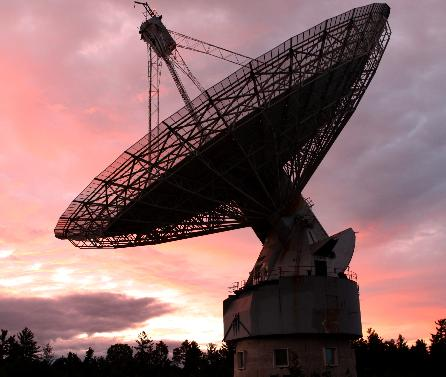
\includegraphics[width=4.4in]{Figures/IMG-7749-ARO-crop.JPG}

\frame{
\vspace{-0.5in}
\begin{center}  
%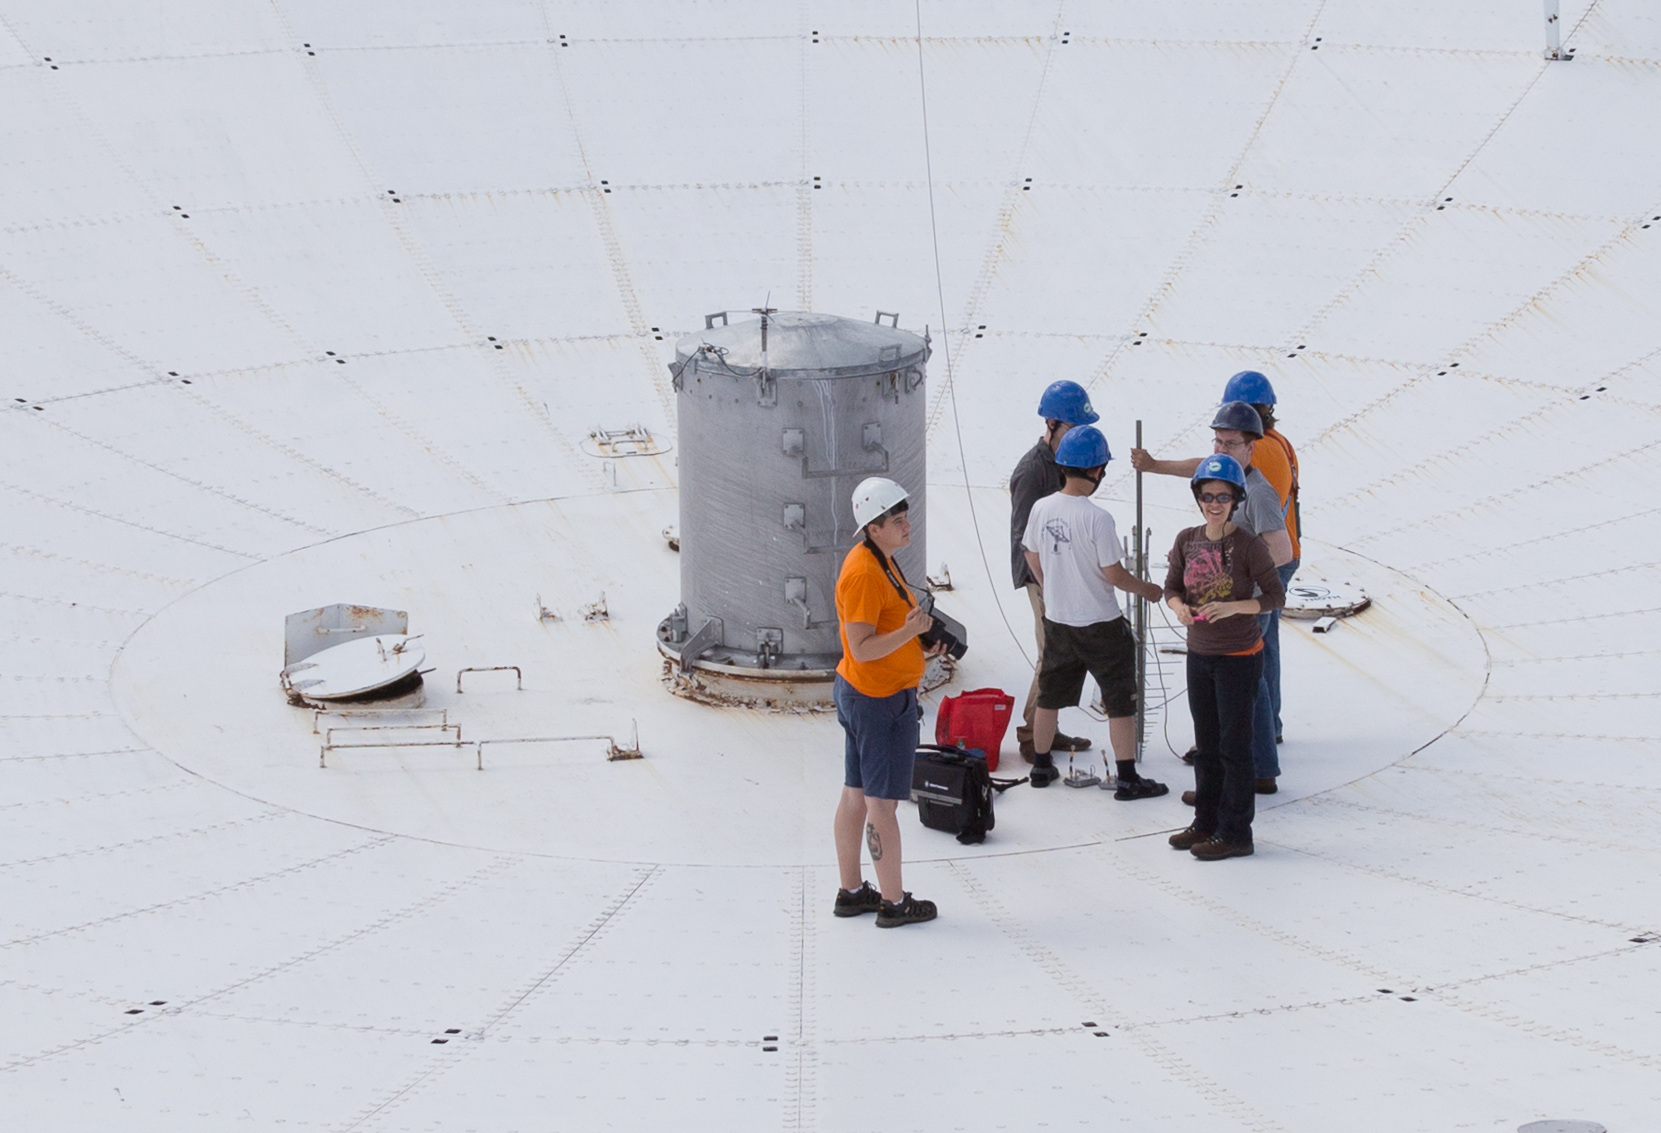
\includegraphics[width=4.4in]{Figures/IMG-0438-by-Andre-cropped.jpg}
\end{center}
\begin{picture}(320,250)
\put(-50,60){
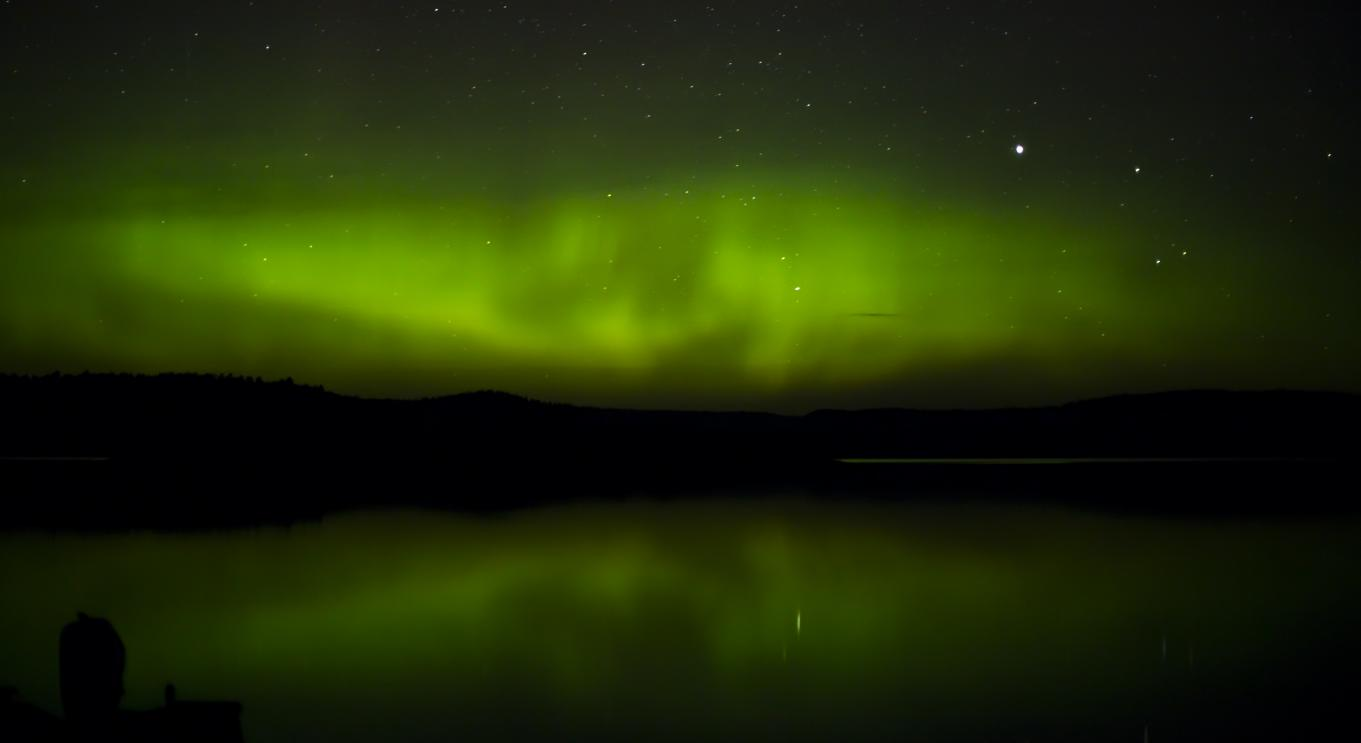
\includegraphics[width=5.5in]{Figures/traverse-aurora.jpg}}
\end{picture}
\vspace{-4in}
\\
image credit: Andre Recnik
\\
\vspace{1in}
\titlepage
}


%\section*{Introduction}
\section{Introduction}

\begin{comment}
  \subsection{Outline}

  \frame{
    \frametitle{Outline}
    \tableofcontents
  }
\end{comment}

  \frame{
    \frametitle{Overview}
    \begin{itemize}
      \item phase coherence provides unique precision probes: e.g. LIGO
      \item FRB and pulsar radiation maintains phase coherence in the
        radio band, resulting in interference phenomena
      \item allows coherent VLBI measurements on earth
      \item potential tests of GR, GW, DE, DM, pulsar emission, EoS, 
      \item initial results on FRBs, pulsar emission, scalar gravity
      \item open new opportunity for space VLBI
    \end{itemize}
    \vspace{-.01in}\hspace{2in}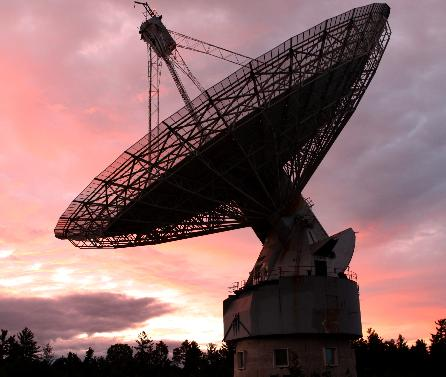
\includegraphics[width=0.3\textwidth]{Figures/IMG-7749-ARO-crop.JPG}
  }


  \frame{
    \frametitle{Scintillometry}
PSR B0834+06: 
$D_S=620$pc, 
$D_L=389/415$pc
{\tiny Brisken+2010, Liu+2016}

%\vspace{-0.95in}
\hspace{1.75in}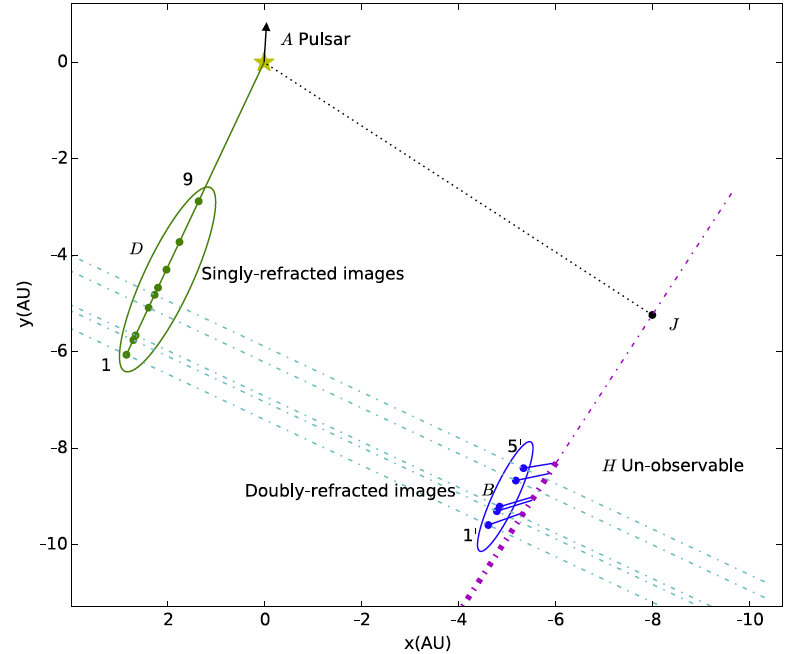
\includegraphics[width=0.7\textwidth]{Figures/liu-lens.png} 
  }

  \frame{
    \frametitle{Applications}
    \begin{itemize}
      \item cosmic telescope: picoarcsecond astrometry of magnetospheres
      \item measured 1km deflection of PSR B0834+06 emission, initial
        results for crab, black widow
      \item likely connection to Extreme Scattering Events
      \item potential for precision distances to pulsars, increased
        PTA sensitivity, accurate GW localization.
    \end{itemize}
  }
 

\end{document}
